% called by main.tex
\chapter{Cơ sở lý thuyết và thuật toán}
\label{ch::chapter2}

CSMA/CA (Carrier Sense Multiple Access with Collision Avoidance) là một phương pháp truy cập truyền 
thông được sử dụng trong mạng không dây để giảm thiểu va chạm dữ liệu. Đây là một phương pháp truy 
cập ngẫu nhiên trong đó các thiết bị trong mạng truyền thông sẽ kiểm tra tình trạng kênh trước khi 
truyền dữ liệu và thực hiện các biện pháp để tránh xung đột dữ liệu.

Nguyên tắc cơ bản khi truy cập của chuẩn IEEE 802.11 là sử dụng cơ chế CSMA/CA– Đa truy cập sử dụng sóng 
mang phòng tránh xung đột. Nguyên tắc này gần giống như nguyên tắc CSMA/CD (Carrier Sense Multiple 
Access Collision Detect) của chuẩn 802.3 (cho Ethernet). Điểm khác ở đây là CSMA/CA nó sẽ chỉ truyền 
dữ liệu khi bên kia sẵn sàng nhận và không truyền hay nhận dữ liệu nào khác trong lúc đó, đây còn gọi 
là nguyên tắc LBT (listening before talking) – nghe trước khi nói.

Theo chuẩn IEEE 802.11, kỹ thuật CSMA/CA được sử dụng tại lớp MAC bởi hàm Distributed Coordination Function (DCF) như trong hình~\ref{fig:mac}.
\begin{figure}[h]
    \centering
    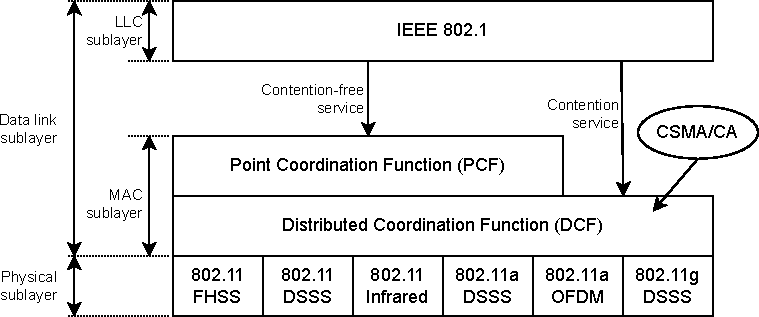
\includegraphics[width=0.85\linewidth]{figures/Chapter2/MAClayer_k2opt.pdf}
    \caption{Lớp MAC trong chuẩn IEEE 802.11}
    \label{fig:mac}
\end{figure}

Quá trình tránh va chạm được thực hiện qua 3 bước: cài đặt thời gian chờ liên gói tin (Interframe Space), khung thời gian
va chạm (Contention window) và xác nhận (Acknowledgments) \cite{nam}.

\begin{figure}[h]
    \centering
    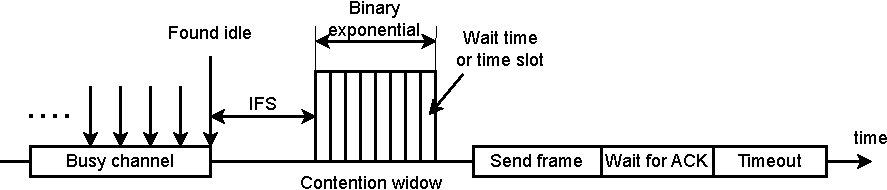
\includegraphics[width=1.1\linewidth]{figures/Chapter2/Procedure_k2opt.pdf}
    %width=
    \caption{Quy trình tránh đụng độ}
    \label{fig:procedure}
\end{figure}

Hình~\ref{fig:procedure} thể hiện quy trình tránh va chạm của kỹ thuật CSMA/CA. Các bước thực hiện được mô tả như sau:
\begin{enumerate}
    \item Interframe Space: đầu tiên, trạm phát cảm nhận kênh truyền và khi phát hiện kênh truyền nhàn rỗi (trống), trì hoãn việc truyền dữ liệu một khoảng thời gian. Nguyên nhân là vì tại thời điểm phát hiện kênh nhàn rỗi, có thể có một trạm ở khoảng cách xa hơn bắt đầu truyền dữ liệu gói tin đó chưa đến. IFS là khoảng thời gian chờ nếu có một trạm khác đang truyền. Sau khoảng thời gian IFS mà kênh truyền vẫn nhàn rỗi, dữ liệu bắt đầu được truyền. Biến IFS có thể đánh dấu ưu tiên cho những trạm hoặc loại dữ liệu truyền. Dữ liệu càng được ưu tiên thì IFS càng ngắn \cite{nam}.
    \item Contention window: Khoảng thời gian được chia thành nhiều khe thời gian (slot time). Trạm nào đã sẵn sàng gửi dữ liệu sẽ chọn một vị trí ngẫu nhiên và đó sẽ là thời gian chờ. Số lượng khe thời gian tùy thuộc vào chiến lược lùi lại theo cấp số nhân nhị phân (binary exponential back-off strategy). Điều này có nghĩa là sau mỗi lần trạm phát không tìm được kênh nhàn rỗi, nó sẽ gấp đôi thời gian chờ. Trạm phát sẽ cảm nhận kênh truyền khi thời gian chờ kết thúc. Bộ đếm thời gian chờ chỉ khởi động lại khi đã phát hiện kênh truyền nhàn rỗi \cite{nam}.
    \item Acknowledgments: gói tin sẽ được gửi khi 2 quy trình trên được thỏa yêu cầu. Sau đó, trạm phát sẽ chờ gói tin xác nhận từ phía nhận để tiếp tục kết nối và truyền dữ liệu \cite{nam}.
\end{enumerate}

Để thực hiện mô phỏng cho cơ chế CSMA/CA trong thực tế, một mô hình đại diện gồm 3 trạm thu phát tín hiệu được sử dụng. Cơ chế hoạt động của CSMA/CA có thể được mô tả như sau:
\begin{enumerate}
    \item Khi một thiết bị muốn truyền dữ liệu, nó sẽ kiểm tra xem kênh truyền có sẵn hay không (Carrier Sense).
    \item Nếu kênh truyền rảnh, thiết bị sẽ bắt đầu truyền dữ liệu.
    \item Phía phát sẽ chờ gói tin xác nhận từ phía thu để quyết định các bước truyền dữ liệu tiếp theo.
    \item Trong khi đó, các trạm khác tiếp tục quá trình lắng nghe kênh truyền để phát hiện quy trình truyền đã kết thúc.
\end{enumerate}

\begin{figure}[h]
    \centering
    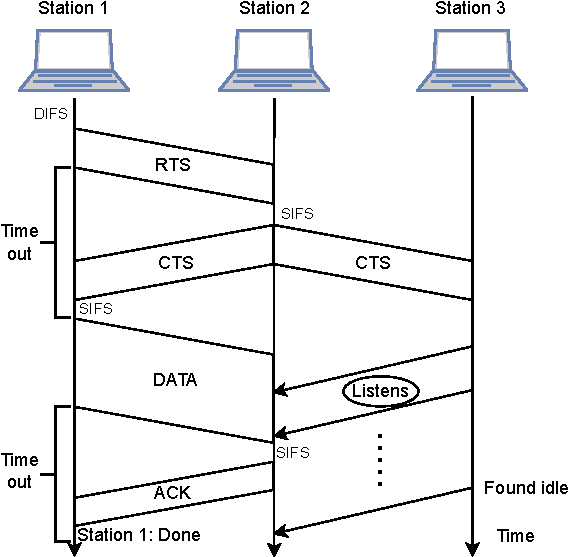
\includegraphics[width=0.7\linewidth]{figures/Chapter2/csma_ca scheme_k2opt.pdf}
    %width=
    \caption{Cơ chế tránh đụng độ với mô hình mạng gồm 3 điểm}
    \label{fig:csmaca}
\end{figure}

Hình~\ref{fig:csmaca} mô tả quy trình CSMA/CA với 3 trạm. Giả sử rằng thời điểm Station 1 truyền dữ liệu kênh truyền đang ở trạng thái nhàn rỗi.
Trong quá trình Station 1 truyền dữ liệu, Station 3 thực hiện việc lắng nghe kênh truyền. Khi Station 1 kết thúc truyền, Station 3 nhận biết kênh truyền 
đã nhàn rỗi và thực hiện quy trình như mô tả ở hình~\ref{fig:procedure}.

% Flow chart lý thuyết

% Flowchart thực tế

Dựa trên ý tưởng lưu đồ thuật toán ở hình \ref{fig:flowchart}, lưu đồ thuật toán đã được xây dựng lại cho phần mô phỏng ở chương \ref{ch::chapter3} như trong hình \ref{fig:flowcode}. Khi hệ thống phát hiện
xung đột, có 5 chiến lược (Back-off Strategy) được đưa ra như sau:
\begin{itemize}
    \item Strategy 1: Tăng CW = CW * 2 khi xảy ra xung đột và đặt lại CW = CWmin khi truyền dữ liệu thành công.
    \item Strategy 2: Tăng CW = CW + 2 khi xảy ra xung đột và giữ nguyên CW khi truyền dữ liệu thành công.
    \item Strategy 3: Tăng CW = CW * 2 khi xảy ra xung đột và giữ nguyên CW khi truyền dữ liệu thành công.
    \item Strategy 4: Tăng CW = CW + 2 khi xảy ra xung đột và giảm CW = CW - 2 khi truyền dữ liệu thành công.
    \item Strategy 5: Tăng CW = CW * 2 khi xảy ra xung đột và giảm CW = CW - 2 khi truyền dữ liệu thành công.
\end{itemize}


\begin{figure}[h]
    \centering
    \begin{subfigure}[h]{0.45\linewidth}
        \centering
        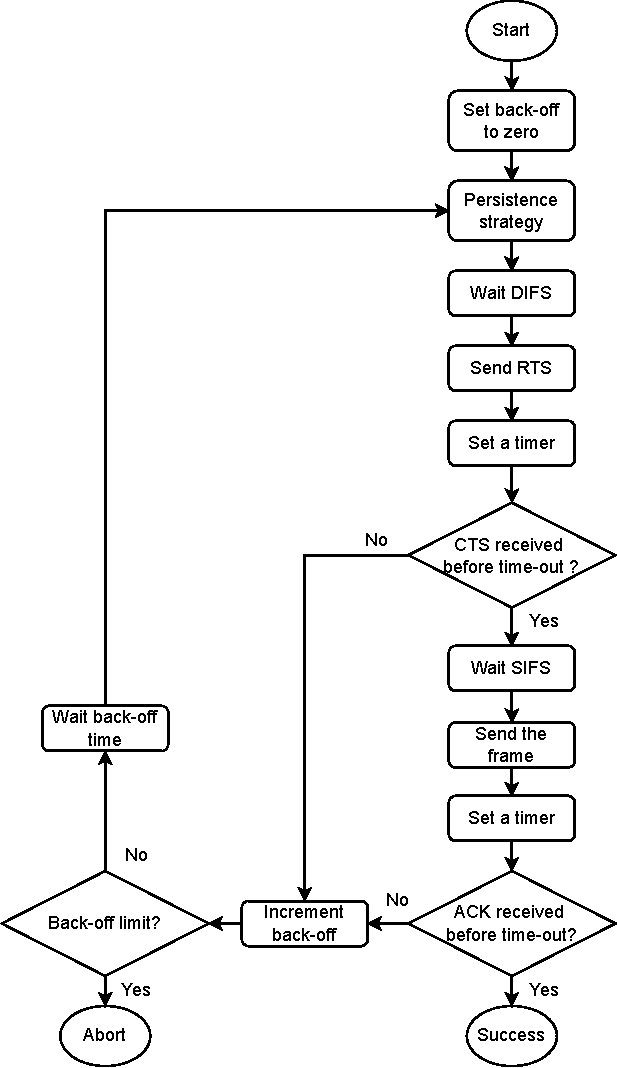
\includegraphics[width=1.13\linewidth]{figures/Chapter2/flowchart_k2opt.pdf}
        \caption{Lưu đồ thuật toán dự trên lý thuyết}
        \label{fig:flowchart}
    \end{subfigure}
    \hspace{0.05\linewidth} % Adjust the spacing between subfigures
    \begin{subfigure}[h]{0.45\linewidth}
        \centering
        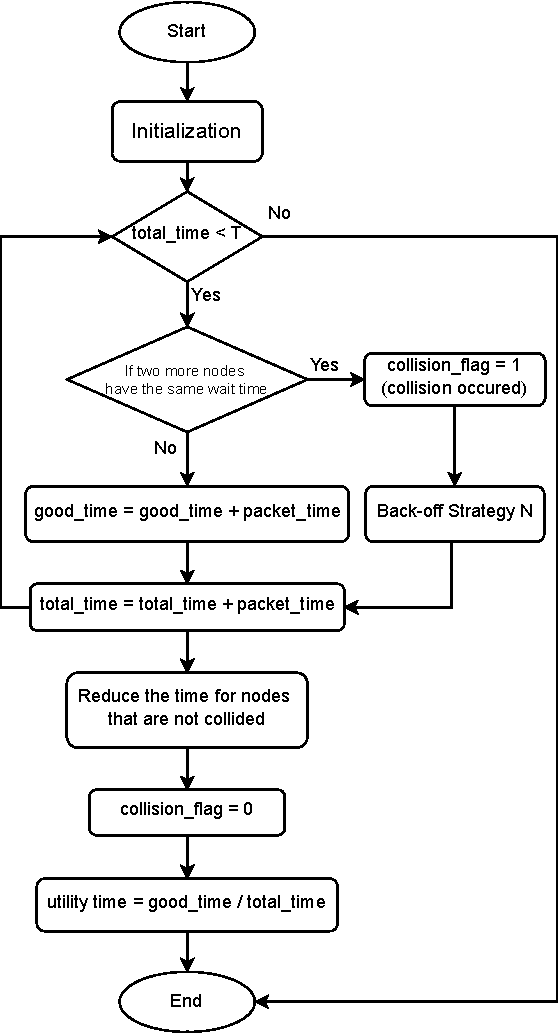
\includegraphics[width=1.1\linewidth]{figures/Chapter2/code_flow.pdf}
        \caption{Lưu đồ thuật toán dự trên mô phỏng}
        \label{fig:flowcode}
    \end{subfigure}

    \caption{Lưu đồ thuật toán }
    \label{fig:csmacaflowchart}
\end{figure}


